\section{Documentation}
\subsection{How the Project Works}
\subsubsection{Overview}
This project works by combining the power of Robot Operating System (ROS), the Qt framework, and Python to make a simple (for what it is), fast, easy to modify, and easier to understand piece of software to act as the front end for the Mars Rover. PyQt is used to load and show the UI and give the software programmatic access to GUI elements. It also provides intelligent multi-threading with easy to use cross-thread communication pipelines. The use of python has allowed our team to write this code in a fraction of the time it would have taken in another language such as C++. ROS is the framework that the Rover is running and is based around the concept of abstracting everything into ROS topics. These topics allow for easy sending and receiving of control and status information in a way that is standardized instead of having to use a custom network control protocol.

\subsubsection{Low bandwidth communications}
As the Rover is going to be at long range at many times, having as small of communication packets as possible is a priority. This helps keep control, video, and status information smooth and consistent. In order to facilitate this, the ground station and Rover both are using a package called nimbro\_network that allows for compression of ROS topics and also allows for us to choose between a TCP and UDP transport layer. Non-critical data that we want fast gets sent with compression over UDP and includes video data from the Rover and live drive commands from the ground station. Important and/or infrequent data is sent with or without compression depending and using the TCP transport. Data sent using TCP includes status information from the Rover and, in the future, waypoints and autonomy control. 

\subsubsection{Program Logical Structuring}
To make the ground station software easier to modify and understand, it has been broken down into logical hierarchies. At the core of the ground station source folder are the Framework and Resources folders. The Resources folder contains all of the static assets for the application such as image files and the UI files that determine how the GUI visually looks. The Framework folder contains all of the logical sub-systems of the software such as VideoSystems, InputSystems, and MappingSystems. By separating all systems out like this, it makes it easy to know which files need to be looked at when fixing or adding to the ground station. At the root of the source folder is "ground\_station.py", the launcher file for the whole application. Under normal conditions, this file only needs to be modified if a new threaded class is being added for additional functionality. This file handles launching of the software, displaying the GUI, and management of the startup and shutdown of all running threads.

\subsubsection{Threading \& Adding Classes}
As this is a very large program with many systems running concurrently it has required the use of many threaded classes. To abstract away many of the complexities of this, the ground station main launcher file contains a method called add\_thread used to spin up a new threaded class from the Framework folder when one is made. This method also handles the graceful shutdown of the software when quit. In order for graceful shutdown, all of the program's child threads must not be running when the main launcher thread exits. If this is not the case, the application may hang or maintain unwanted connections in the background after it seems like it has exited. Anyone wishing to add new functionality to the GUI in a new file should copy an existing threaded class to use as a baseline.

\subsubsection{ROS in Python}
ROS is a large part of why this software has been much easier to write than it could have been. In Python, the ROS subsystem can be accessed by importing rospy and calling rospy.init to tell ROS that we have a new node running. At this point, topics can be subscribed to by giving it the topic path and a the data type of the topic. Conversely, to broadcast a new topic message, a publisher is made by providing the topic path, data type, and queue size. To actually broadcast a message, you create a new instance of the data type, fill it with the desired data, and use the publisher's ".publish()" method to send it. In our software, these topics are used for all communications to and from the Rover. Absolutely no custom communication methods are used to interface between the Rover and ground station. An important note about the ROS messages used are that most of these messages are custom defined. In order for rospy and python to know the required information about a custom message, the ROS package containing the message define must be built as part of the local catkin workspace. This is the reason that the ground station's setup script includes many packages other than for just launching the ground station. The extra packages give us access to custom messages needed for understanding status messages and sending drive commands.

\subsubsection{ROS Topic / Classes Block Diagram}
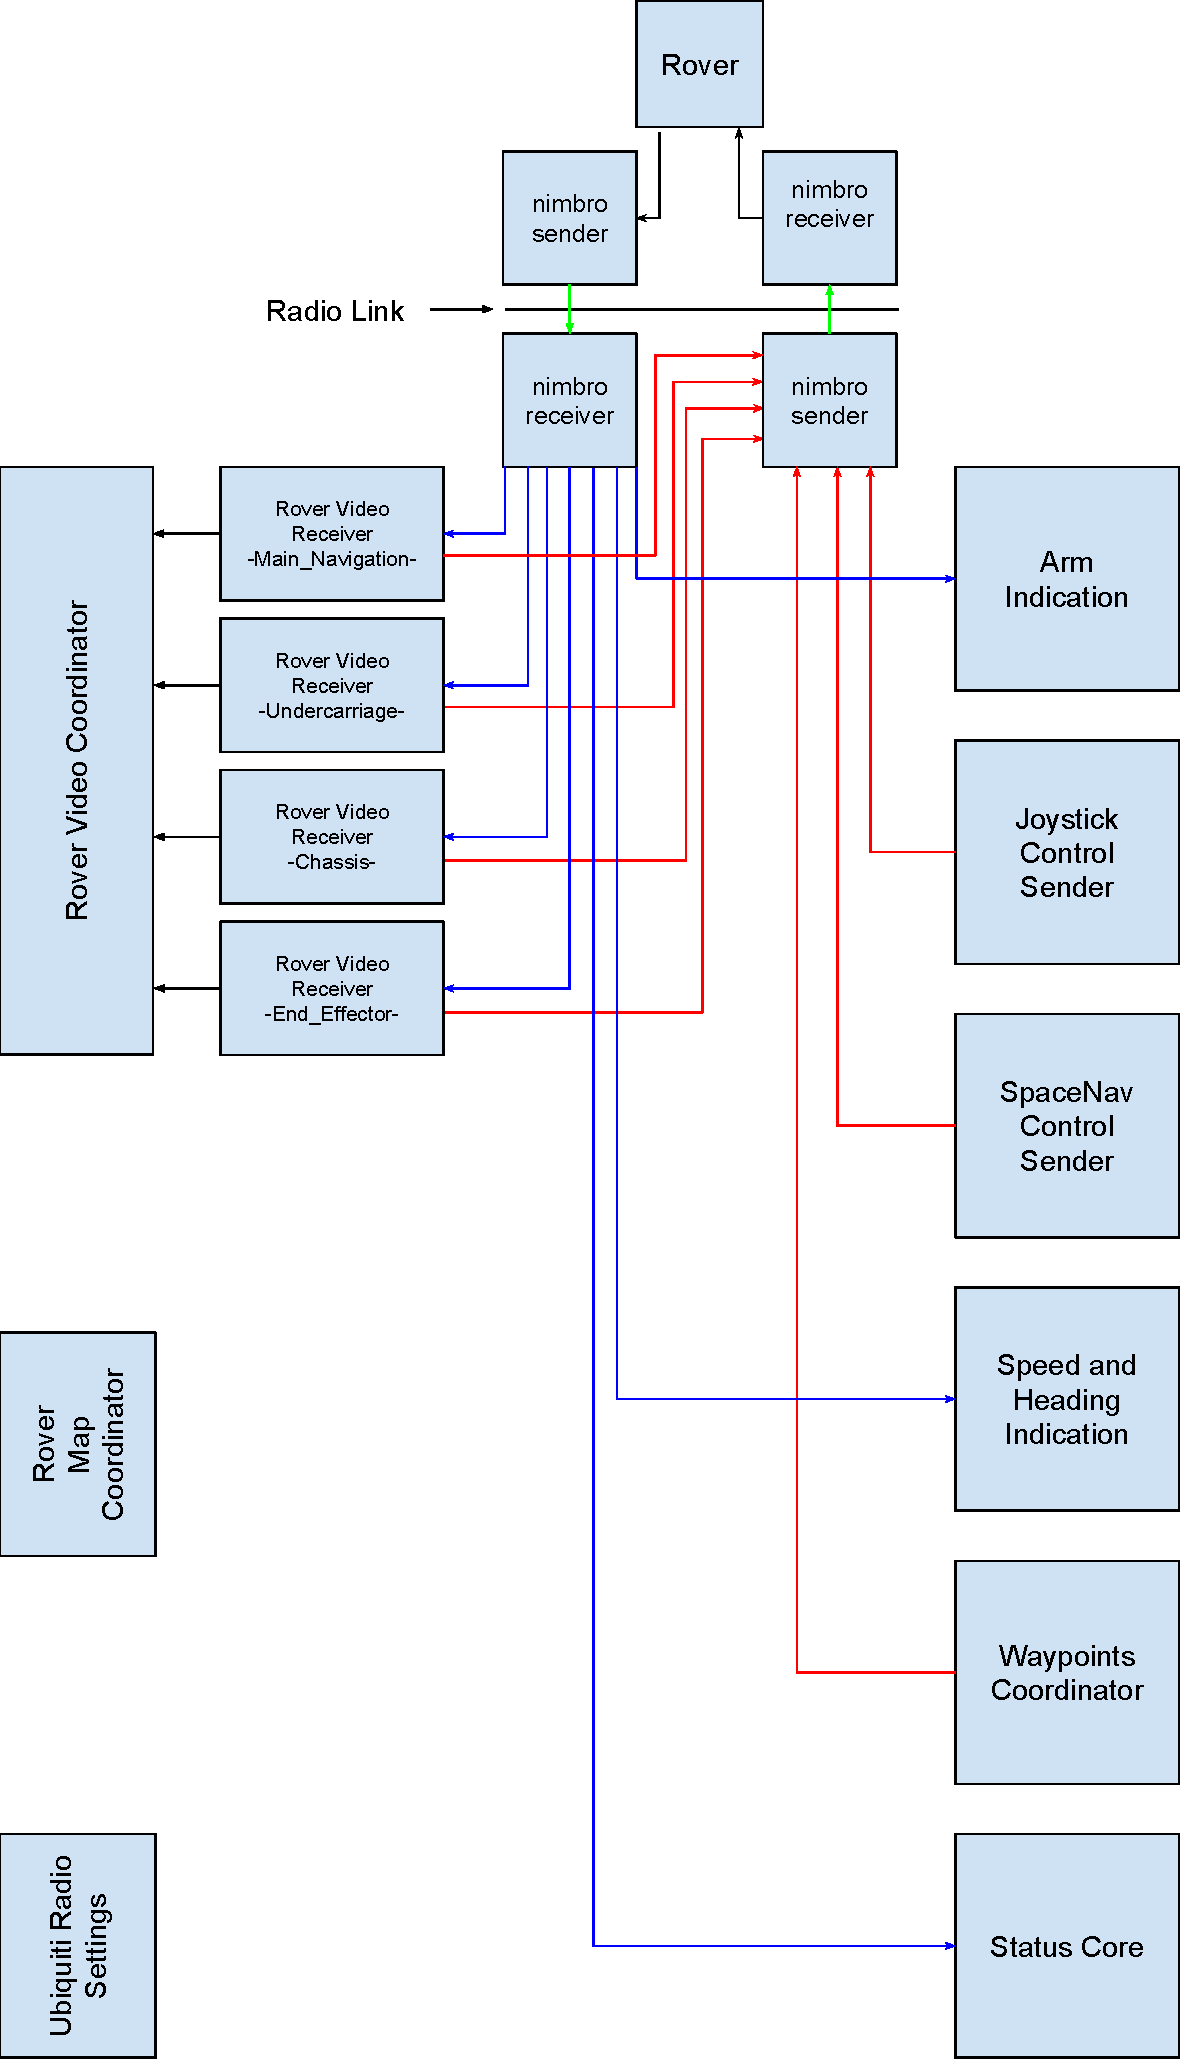
\includepdf[pages=-, scale=0.98]{07-documentation/Rover_Ground_Station_Block_Diagram.pdf}


\subsection{System Requirements}
\subsubsection{Hardware}
\begin{itemize}
\item 1x Computer running Ubuntu 16.04 LTS
	\begin{itemize}
	\item Intel core i5 or i7 equivalent processor
    \item 4GB+ Ram
    \item Minimum two display outputs
	\end{itemize}
\item 2x 1080p Monitors
\item 1x USB Joystick
\item 1x SpaceNav Mouse
\item 1x USB Keyboard
\item 1x USB Mouse
\end{itemize}

\subsubsection{Software / OS}
\begin{itemize}
\item \href{http://wiki.ros.org/kinetic/Installation}{ROS Kinetic}
\item \href{https://www.python.org/}{Python 2.X} with the following packages:
	\begin{itemize}
	\item PyQt5
    \item qdarkstyle
    \item inputs
    \item spnav
    \item Pillow
    \item paramiko
    \item OpenCV 2
    \item qimage2ndarray
    \item numpy
	\end{itemize}
\item Set the computer to an IP address of 192.168.1.15
\end{itemize}


\subsection{How to Install}
\begin{enumerate}
\item Create and \href{http://wiki.ros.org/catkin/Tutorials/create_a_workspace}{setup a catkin workspace} at "$\sim$/catkin\_workspace"
\item Add "source /home/[username]/catkin\_workspace/devel/setup.bash" to the end of your ".bashrc" file, replacing "[username]" with your account's username
\item Create the directory "$\sim$/Github" and clone the \href{https://github.com/OSURoboticsClub/Rover_2017_2018}{Rover\_2017\_2018} repository into it
\item Run the setup script at "$\sim$/Github/Rover\_2017\_2018/software/ground\_station\_setup.sh" to have the proper packages symbolically linked into your new catkin environment and for catkin\_make to be run automatically against it
\item If the catkin\_make process at the end of the script completes with no errors, you're ready to launch the ground station
\end{enumerate}


\subsection{How to Run}
\begin{enumerate}
\item Ensure all hardware from the requirements section above is plugged in
\item Ensure there is a network connection between the ground station computer and Rover
\item Open a terminal and run "roslaunch rover\_main ground\_station.launch"
\item The ground station should launch in full screen across both monitors
\item Press "ctrl-q" at any time to quit the application
\end{enumerate}


\subsection{User Guides}
\subsubsection{Client Requested Quickstart Guide}
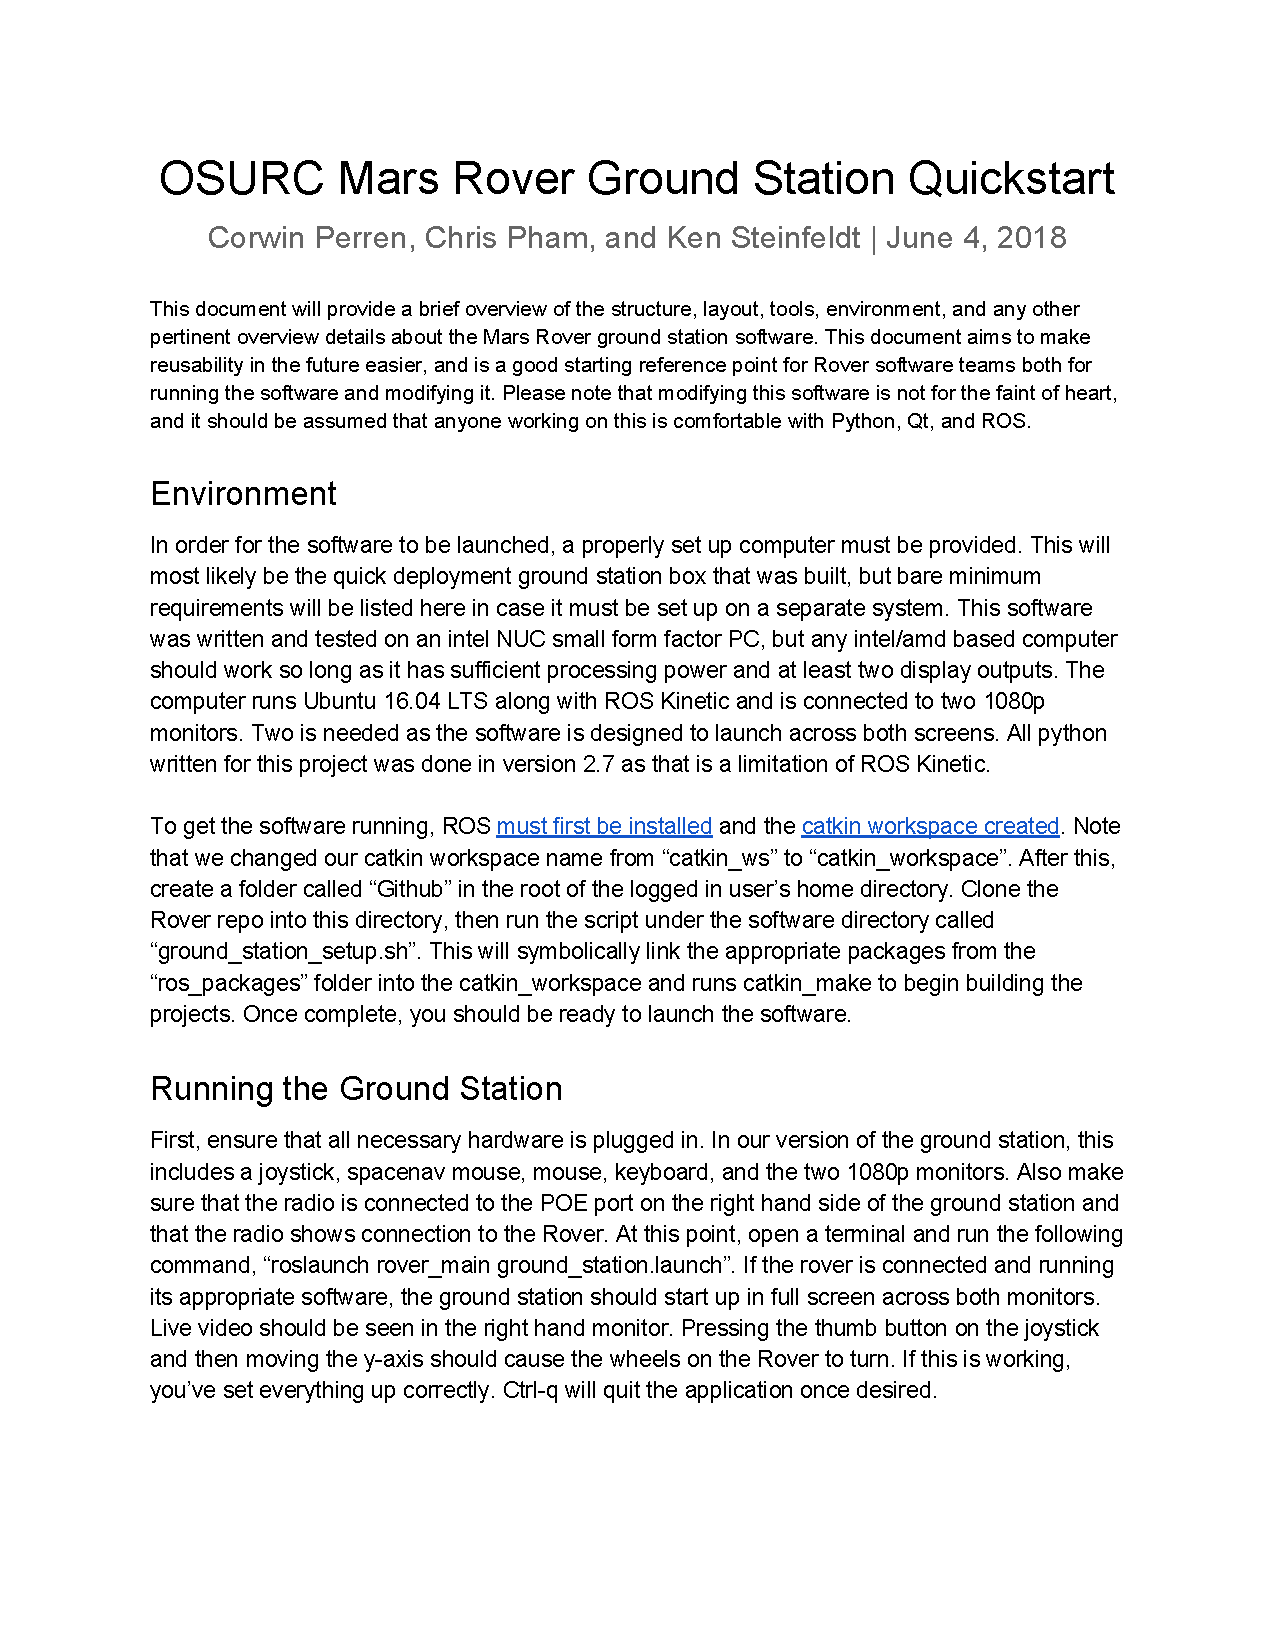
\includepdf[pages=-, frame=true, scale=0.95]{07-documentation/Ground_Station_Quickstart.pdf}